% 拉普拉斯变换的性质
% 拉普拉斯变换|导数|积分|位移|卷积

\pentry{拉普拉斯变换\upref{LapTra}}

前面我们介绍了拉普拉斯变换,那么这个变换到底给我们带来了什么特别的好处呢?我们下面就来看一下它到底具有哪些性质.

\subsection{线性性质}


若$\mathscr L[f_1(t)] = \bar f_1(p)$, $\mathscr L[f_2(t)] = \bar f_2(p)$,则
\begin{equation}
\mathscr L[c_1f_1(t)+c_2f_2(t)] = c_1\bar f_1(p) + c_2\bar f_2(p)
\end{equation}

证明起来也十分容易.
\begin{equation}
\begin{aligned} \mathscr L[c_{1} f_{1}(t)+c_{2} f_{2}(t)] & = \int_{0}^{\infty}\left[c_{1} f_{1}(t)+c_{2} f_{2}(t)\right] \mathrm{e}^{-\rho t} \mathrm{d} t \\ &=\int_{0}^{\infty} c_{1} f_{1}(t) \mathrm{e}^{-p t} \mathrm{d} t+\int_{0}^{\infty} c_{2} f_{2}(t) \mathrm{e}^{-\rho t} \mathrm{d} t \\ &=c_{1} \bar{f}_{1}(p)+c_{2} \bar{f}_{2}(p) \end{aligned}
\end{equation}

它能让我们干什么呢?我们可以把未知的函数拆成已知函数的线性组合,相加它们的拉普拉斯变换来得到所要的未知函数的拉普拉斯变换.例如:
\begin{example}{线性性质的应用}
求$\mathscr L[\sin \omega t]$,$\omega$为常数.

我们知道
\begin{equation}
\sin \omega t=\frac{1}{2 \mathrm{i}}\left(\mathrm{e}^{\mathrm{i} \omega t}-\mathrm{e}^{-\mathrm{i} \omega t}\right)
\end{equation}
所以有
\begin{equation}
\begin{aligned} \mathscr{L}[\sin \omega t] &=\mathscr{L}\left[\frac{1}{2 \mathrm{i}}\left(\mathrm{e}^{\mathrm{i} \omega t}-\mathrm{e}^{-\mathrm{i} \omega t}\right)\right]=\frac{1}{2 \mathrm{i}} \mathscr{L}\left[\mathrm{e}^{\mathrm{i} \omega t}\right]-\frac{1}{2 \mathrm{i}}\mathscr{L}\left[\mathrm{e}^{-\mathrm{i} \omega t}\right] \\ &=\frac{1}{2 \mathrm{i}}\left[\frac{1}{p-\mathrm{i} \omega}-\frac{1}{p+\mathrm{i} \omega}\right] \\ &=\frac{\omega}{p^{2}+\omega^{2}} \quad(\Re p>0) \end{aligned}
\end{equation}

同理可得
\begin{equation}
\mathscr{L}[\cos \omega t]=\frac{p}{p^{2}+\omega^{2}} \quad(\operatorname{Re} p>0)
\end{equation}
\end{example}

\subsection{导数定理}

拉普拉斯变换的导数定理是说:
\begin{equation}
\mathscr L[f'(t)]=p\bar f(p)-f(0)
\end{equation}

证明同样直接积分就可以了.

\begin{equation}
\begin{aligned} \mathscr L[f^{\prime}(t)] & = \int_{0}^{\infty} f^{\prime}(t) \mathrm{e}^{-p t} \mathrm{d} t=\int_{0}^{\infty} \mathrm{e}^{-p t} \mathrm{d} f \\ &=\left[\mathrm{e}^{-p t} f(t)\right]_{0}^{\infty}-\int_{0}^{\infty} f(t) \mathrm{d}\left(\mathrm{e}^{-p t}\right) \end{aligned}
\end{equation}
取$\Re p>\sigma$,有$\lim_{t\to\infty}\mathrm{e}^{-pt}f(t)=0$.于是可得
\begin{equation}
\begin{aligned} \mathscr L[f^{\prime}(t)] & = -f(0)-\int_{0}^{\infty} f(t) \mathrm{d}\left(\mathrm{e}^{-\rho t}\right)=p \int_{0}^{\infty} f(t) \mathrm{e}^{-p t} \mathrm{d} t-f(0) \\ &=p \bar{f}(p)-f(0) \quad\left(\operatorname{Re} p>\sigma_{0}\right) \end{aligned}
\end{equation}

我们还可以推广到高阶导数的情形:
\begin{equation}
\mathscr L[f^{(n)}(t)] = p^{n} f(p)-p^{n-1} f(0)-p^{n-2} f^{\prime}(0)-\cdots-p f^{(n-2)}(0)-f^{(n-1)}(0)
\end{equation} 

有了导数定理,让我们来想想导数的逆运算——积分!有没有积分定理呢?有!

\subsection{积分定理}
\begin{equation}
\mathscr L\left[\int_{0}^{t} \psi(\tau) \mathrm{d} \tau \right]=\frac{1}{p} \mathscr{L}[\psi(t)]
\end{equation}

证明其实也一样简单.设$\displaystyle f(t)=\int_{0}^{t} \psi(\tau) \mathrm{d} \tau$,对$f(t)$应用导数定理,可知:
\begin{equation}
\mathscr[f^{\prime}(t)]=p \mathscr{L}[f(t)]-f(0)=p \mathscr{L}[f(t)]
\end{equation}
所以也就有
\begin{equation}
\frac{1}{p} \mathscr{L}[\psi(t)]=\mathscr{L}[f(t)]=\mathscr{L}\left[\int_{0}^{t} \psi(\tau) \mathrm{d} \tau\right]
\end{equation}
这也就证明了定理.
 
\subsection{相似性定理}
\begin{equation}
\mathscr{L}[f(at)]=\frac{1}{a} \bar{f}\left(\frac{p}{a}\right)
\end{equation}
证明留作练习.

\subsection{位移定理}
\begin{equation}
\mathscr{L}[\mathrm{e}^{-\lambda t} f(t)]= \bar{f}(p+\lambda)
\end{equation}

这个证明也十分简单,留作练习.

\subsection{延迟定理}
\begin{equation}
\mathscr{L}\left [f\left(t-t_{0}\right)\right] =\mathrm{e}^{-p t_{0}} \bar f(p)
\end{equation}

用换元积分即可证明.具体来说:
\begin{equation}
\mathscr L\left [f\left(t-t_{0}\right)\right] =\int_{0}^{\infty} f\left(t-t_{0}\right) \mathrm{e}^{-p t} \mathrm{d} t
\end{equation}
我们知道在$t<0$时,默认$f(t)$都是$0$.那么我们做积分的时候,时间可以改为从$t_0$开始积分.也就是说:
\begin{equation}
\mathscr L\left [f\left(t-t_{0}\right)\right] =\int_{t_0}^{\infty} f\left(t-t_{0}\right) \mathrm{e}^{-p t} \mathrm{d} t
\end{equation}
作换元$\xi=t-t_0$,那么就有
\begin{equation}
\begin{aligned} \mathscr L\left[f\left(t-t_{0}\right)\right] &=\int_{0}^{\infty} f(\xi) \mathrm{e}^{-p\left(\xi+t_{0}\right)} \mathrm{d} \xi=\mathrm{e}^{-p t_{0}} \int_{0}^{\infty} f(\xi) \mathrm{e}^{-p \xi} \mathrm{d} \xi \\ &=\mathrm{e}^{-p t_{0}} \bar{f}(p) \end{aligned}
\end{equation}

\subsection{卷积定理}

卷积定理是说,若$\mathscr L[f_1(t)] = \bar f_1(p), \mathscr L[f_2(t)] = \bar f_2(p)$,则
\begin{equation}
\mathscr L[f_{1}(t) * f_{2}(t) ]= \bar{f}_{1}(p) \bar{f}_{2}(p)
\end{equation}

下面我们来证明它.这个证明稍复杂一些,毕竟它是二重积分:
\begin{equation}
\begin{aligned} & \mathscr{S}\left[f_{1}(t) * f_{2}(t)\right] \\=& \int_{0}^{\infty} f_{1}(t) * f_{2}(t) \mathrm{e}^{-p t} \mathrm{d} t \\=& \int_{0}^{\infty}\left[\int_{0}^{t} f_{1}(\tau) f_{2}(t-\tau) \mathrm{d} \tau\right] \mathrm{e}^{-p t} \mathrm{d} t \end{aligned}
\end{equation}
\begin{figure}[ht]
\centering
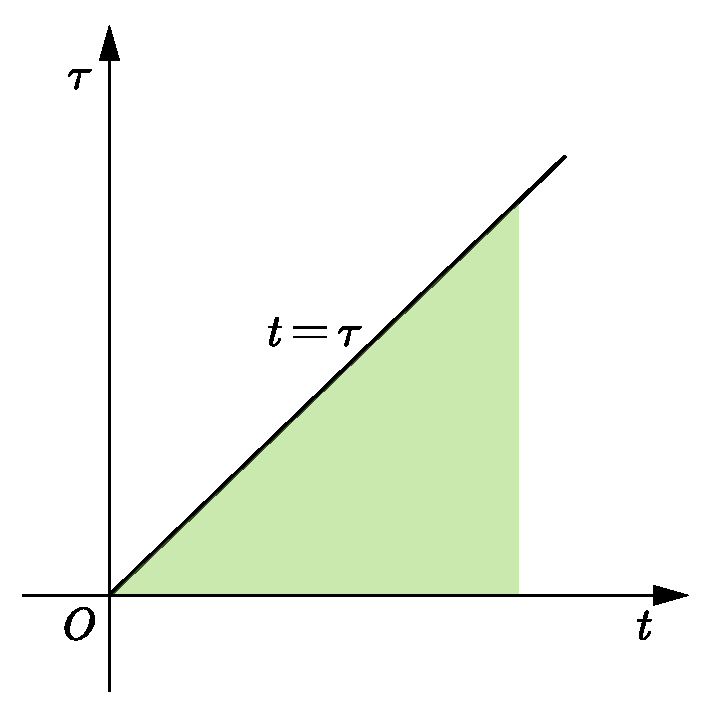
\includegraphics[width=6cm]{./figures/ProLap_1.pdf}
\caption{积分限} \label{ProLap_fig1}
\end{figure}
我们需要交换积分次序,首先我们来看一下积分区域,它就是\autoref{ProLap_fig1} 中的绿色区域.由此可见,现在改变积分次序,就是说
\begin{equation}
\begin{aligned} & \mathscr{L}\left[f_{1}(t) * f_{2}(t)\right] \\=& \int_{0}^{\infty}\left[\int_{\tau}^{\infty} f_{2}(t-\tau) \mathrm{e}^{-p t} \mathrm{d} t\right] f_{1}(\tau) \mathrm{d} \tau \end{aligned}
\end{equation}
作换元,$\xi=t-\tau$,那么就有
\begin{equation}
\begin{aligned} \mathscr{L}\left[f_{1}(t) * f_{2}(t)\right] &=\int_{0}^{\infty}\left[\int_{0}^{\infty} f_{2}(\xi) \mathrm{e}^{-p \xi} \mathrm{d} \xi\right] f_{1}(\tau) \mathrm{e}^{-p \tau} \mathrm{d} \tau \\ &=\int_{0}^{\infty} f_{1}(\tau) \mathrm{e}^{-p \tau} \mathrm{d} \tau \int_{0}^{\infty} f_{2}(\xi) \mathrm{e}^{-p \xi} \mathrm{d} \xi \\ &=\bar{f}_{1}(p) \bar{f}_{2}(p) \end{aligned}
\end{equation}

\begin{exercise}{}
求下列函数的拉普拉斯变换.

\begin{enumerate}
\item \begin{equation}
\text { sh } \omega t, \quad \text { ch } \omega t
\end{equation}
\item \begin{equation}
\mathrm{e}^{-\lambda t} \sin \omega t, \quad \mathrm{e}^{-\lambda t} \cos \omega t
\end{equation}
\item \begin{equation}
\frac{1}{\sqrt{\pi t}}
\end{equation}
\item \begin{equation}
\delta(t-\tau)
\end{equation}
\end{enumerate}
\end{exercise}